%!TEX root=../draft.tex
%\vspace{-6pt}
\section{Linear TM Overlay}
\label{ch3_arch}

%\subsection{Data Streaming Model}
While overlays with a general-purpose mesh-based interconnect allow for flexible communication between each FU, they introduce a significant resource overhead associated with the routing network. 
In many cases, a simple linear interconnect structure can be used instead. In a TM overlay, this reduces the highly flexible interconnect to a direct connection between FUs, as in Fig.~\ref{pipelines}, and allows data flow graph (DFG) nodes from the same scheduling time step to be allocated to individual FUs~\cite{li2016area}.
The linear overlay consists of a streaming data interface made up of Distributed RAM (DRAM) acting as a FIFO, which feeds the cascade of time-multiplexed FUs, with another DRAM-based FIFO at the output.
Tasks are scheduled to the overlay using ASAP scheduling, with nodes at the same (horizontal) level allocated to a single FU.
For example, Fig.~\ref{code} shows the medical imaging `gradient' benchmark~\cite{cong2014fully}, while Fig.~\ref{dfg} shows the resulting DFG.
This example requires 4 FU stages, where the first stage contains 4 subtract operations which would execute on the first FU, then the 4 multiplication operations execute on the second FU, and so on.


\begin{figure}[b]
	\centering
	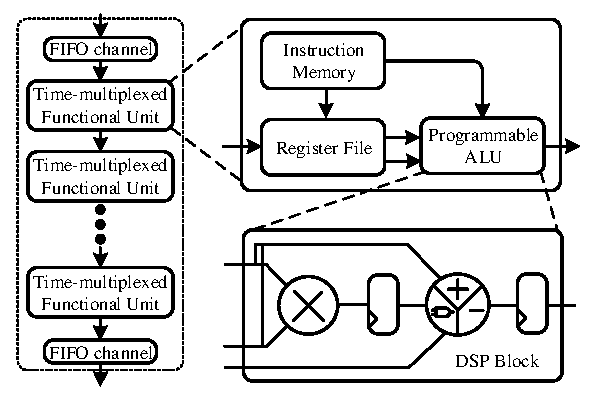
\includegraphics[width=7.5cm]{figures/pipelines_new.pdf}
	\caption{A linear TM overlay.}
	\label{pipelines}
\end{figure}

\begin{figure}[t]
	\centering
	\begin{subfigure}[t]{0.2\textwidth}
		\centering
		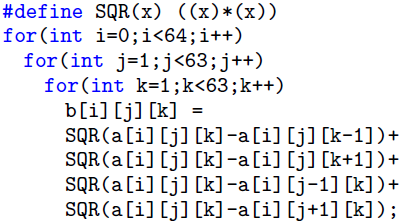
\includegraphics[width=4.6cm]{figures/code.png}
		\caption{C Source Code}
		\label{code}
	\end{subfigure}
	~~
	\begin{subfigure}[t]{0.24\textwidth}
		\centering
		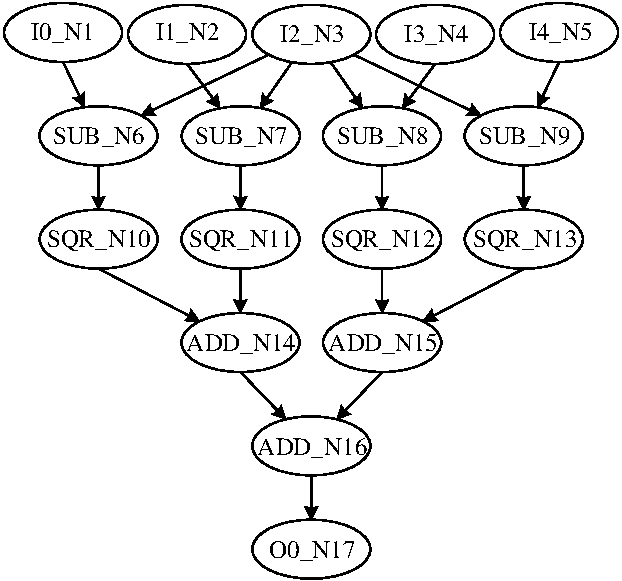
\includegraphics[width=4cm]{figures/DFG.pdf}
		\caption{Data Flow Graph}
		\label{dfg}
	\end{subfigure}
	\caption{The `gradient' benchmark.}
	\label{dfgs}
\end{figure} 


The FU uses the same principle as the iDEA DSP-based processor~\cite{cheah2012idea}, and requires 1 DSP block, 160 LUTs and 293 FFs and runs at 325 MHz on a Xilinx Zynq XC7Z020.
%Xilinx Zynq XC7Z020-1CLG484C.
The FU consists of a LUTRAM-based instruction memory (IM) and register file (RF), and a DSP-based ALU, as shown in Fig.~\ref{fu} (excluding all of the logic in the four dashed boxes). 
%Details of the microarchitecture can be found in~\cite{li2016area}. 

The major advantage of TM overlays is that an application kernel can be mapped to fewer FUs, reducing resource consumption at the expense of II. The example of Fig.~\ref{dfg} can be mapped onto a linear overlay with 4 FUs using ASAP scheduling and has an II of 11, consisting of 5 cycles for data entry, 4 cycles for the 4 subtract operations, 1 cycle for data output and 1 cycle to flush the pipeline.
%For the example shown in Fig.~\ref{dfg} the II is 11, consisting of 5 cycles for data entry, 4 cycles for the 4 subtract operations, 1 cycle for data output and 1 cycle to flush the pipeline.
%%Note that multiplexing the kernel operations of the DFG in Fig. 1(b) to a single FU would result in an II of 17 (5 load, 11 operation, and 1 store), assuming best case execution without NOP insertions, 
By comparison, a spatially configured overlay would have an II of 1, requiring 11 FUs.
However, using ASAP-based scheduling means that the overlay has a depth equal to the critical path of the DFG, and must be re-sized for each new application kernel, thus limiting its usefulness. 
Whereas,  a small linear overlay with a fixed depth that is able to map larger more general purpose compute kernels would be much more useful.
In the next sections, we examine mechanisms to increase the throughput and usability.


\begin{figure*}[!tb]
	\centering
	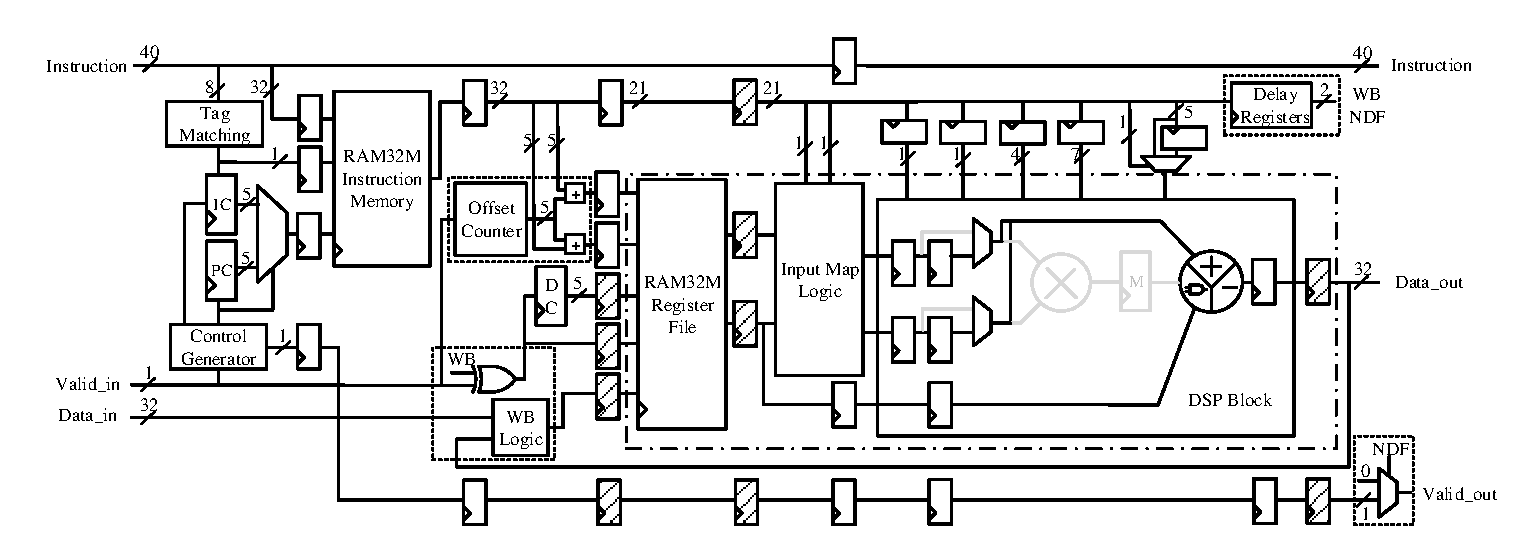
\includegraphics[trim={1cm 0.5cm 1cm 1cm},width=14cm]{figures/FU_WB_new_1.pdf}
	\caption{Proposed time-multiplexed functional unit.}
	\label{fu}
\end{figure*}

\subsection{Architectural Enhancements}
%As discussed earlier, II is one of the critical metrics to determine the throughput of an accelerator for loop kernels.
The II is a critical metric for determining the throughput of an accelerator.
%The II of the overlay in~\cite{li2016area} can be calculated using Equation~\ref{II_V0}. this is significantly higher than that of a spatially configured overlay, and is especially significant for DFGs with a large number of input nodes and operation nodes in the first scheduling stage.
The II of the overlay in~\cite{li2016area} is obtained by the maximum of the number of data load operations plus the number of execution operations with 2 additional clock cycles needed to flush the pipeline among the FUs, as in Equation~\ref{II}.
This is especially large for DFGs with a large number of inputs and operation nodes in the first scheduling stage.
%Equation~\ref{II} gives the II of the overlay in~\cite{li2016area}, which is especially large for DFGs with a large number of inputs and operation nodes in the first scheduling stage. The additional 2 cycles is for flushing the DSP-block pipeline.

\begin{equation}
	II =  \max_{FU} \{\#load + \#op + 2\}
	\label{II}
\end{equation}


\subsubsection{Rotating Register File}
The most obvious way to reduce the II of Equation~\ref{II} is to overlap the loading of input data with instruction execution. 
%Given the simple ASAP operation scheduling shown in~\cite{li2016area}, there is great potential to reduce the II by overlapping the data feeding of RF and the computation of ALU from successive iterations.
Instead of adding additional complexity into the FU to support double-buffering, a rotating register file~\cite{rau1992register} is used to support the overlap of data written into the RF with subsequent instruction execution.
The original design of~\cite{li2016area} used a RAM32M primitive with a dual port configuration (1 read, 1 read/write), whereas the rotating RF version requires a quad port configuration to support 2 reads and 1 write.
The new FU, shown in Fig.~\ref{fu}, includes the offset counter but not the four shaded registers to the left of the RAM32M RF block or the two shaded registers to the right of the DSP block. This design requires 1 DSP block, 196 LUTs, 237 FFs and has a frequency of 334 MHz on a Zynq XC7Z020 (610 MHz on a Virtex-7 VC707).  
%%%The rotating register file allows a new set of input data to be written into later successive locations, which avoids overwriting the current data set.
%Compared with the FU prototype, only an offset counter is added to update the index of read address to avoid the overwritten of successive data set, shown as the left dashed box in Fig.\ref{fu}. 
We refer to this new design as version 1 (V1), and the II is determined as: 
%An example schedule of Fig. 1(b) is given in Section~\ref{ch4_tool} to show the benefit of V1.

\begin{equation}
	II_{V1} =  \max_{FU} \{\#load + 1, \#op + 2\}
	\label{II_V1}
\end{equation}

\noindent where the extra cycle in data load is to separate data blocks.

\subsubsection{Replicating the Stream Datapath}
The II can be reduced, at the expense of an increased data bandwidth requirement, by increasing parallelism.
Replicating the data processing part of the FU (shown within the right dash-dot box) and increasing the data I/O to 64 bits doubles data throughput (halving the II).
This design which reuses the instruction memory and other control circuitry of V1 is called version 2 (V2). It requires 2 DSP blocks, 292 LUTs and 333 FFs, operates at a frequency of 335 MHz and has an II half that of Equation~\ref{II_V1}.

The resource consumption and maximum frequency for the various FU designs on a Zynq XC7Z020 are listed in Table~\ref{FU_table}.
The V1 FU consumes around 22\% more LUTs than that of~\cite{li2016area}, mainly due to the addition of the RAM32M primitive and the offset counter. 
%However, there is an improvement in frequency and a reduction in the number of FFs due to the removal of the registers before the RF.
The resource consumption of V2 is less than twice that of V1, with a similar frequency to V1.

%\begin{equation}
%	II = \{\max_{FU} \{\#load + 1, \#op + 2\}\}/2
%	\label{II_V2}
%\end{equation}


\begin{table}[tb]
	\caption{Comparison of different FU designs.}
	\label{FU_table}
	\centering
	\small
%	\footnotesize
	\begin{tabular}{ccccccc}
		\toprule
		     & ~\cite{li2016area} & V1  & V2  & V3  & V4  & V5  \\ \midrule
		DSPs &         1          &  1  &  2  &  1  &  1  &  1  \\
		LUTs &        160         & 196 & 292 & 212 & 207 & 248 \\
		FFs  &        293         & 237 & 333 & 228 & 163 & 126 \\
		Fmax &        325         & 334 & 335 & 323 & 254 & 182 \\
		IWP  &         --         & --  & --  &  5  &  4  &  3  \\ \bottomrule
	\end{tabular}
\end{table}


%\subsection{Applicability-oriented Architectural Exploration}
%While the performance of the overlay can be improved significantly by reducing the II, it %has to tune to different No. of FUs to fit the DFGs with different depth. 
%A fixed architecture which is able to handle more general applications can be beneficial %to the design productivity, as it save the time for the synthesize of a set of overlay %instances with different requirement of FUs.

\subsubsection{FU Write-back}
The main disadvantage with these overlays is that they are feed-forward only, and thus the overlay depth (and the number of FUs) depends on the critical path of the DFG. 
If output data is written back to the RF, multiple nodes on the DFG critical path could be combined within the same scheduling stage, thus reducing the overlay depth.
%Allowing the output data to be written back to the RF will mean that multiple nodes on the DFG critical path can be combined within the same scheduling stage, thus reducing the overlay depth.
Without write-back, when the application kernel changes the overlay also needs to change, requiring overlay reconfiguration between kernels which significantly impacts the hardware context switch time. 
Thus, a fixed architecture which is able to handle a range of more general kernels would improve execution time when multiple kernels need to be accelerated.

Introducing data write-back is relatively simple and involves feeding the \textit{Data\_out} signal back into the FU and multiplexing it with the \textit{Data\_in} signal, as shown in the lower left dashed box in Fig.~\ref{fu}. 
This requires that the instruction format of~\cite{li2016area} be modified with two extra bits added, a write-back (\textit{WB}) bit and a no data forward (\textit{NDF}) bit. 
Both bits are needed as there is a possibility that the output data will be written back to the RF and bypassed to the next FU stage. Rather than adding two extra bits to the (already) 32-bit instruction, we note that the DSP primitive is only used to support operations with 2 or 3 operands (which means the D port is unused and can be disabled). This means that three bits of the DSP \textit{inmode} field can be hardwired, allowing the use of 1-bit as the \textit{WB} flag, 1-bit as the \textit{NDF} flag, with 1-bit reserved for future use.
The \textit{Valid\_in} signal and the delayed \textit{WB} flag are then used to select between the two different data sources in the write-back logic.

Table~\ref{FU_table} shows the resource utilization, operating frequency and internal write-back path (IWP) for three different implementations of the FU with write-back, referred to as V3, V4 and V5.
The V3 FU is identical to V1, except that the write-back logic is added. That is, it includes all circuitry in Fig.~\ref{fu} apart from the left and right shaded registers.
The IWP is five, comprising one cycle in the RF, one at the register between the RF and the input map logic, and three in the DSP block. This overlay operates at a frequency close to that of the non-WB overlays. 
To reduce the IWP, the registers between the RF RAM32M primitive and the input map logic can be deleted, resulting in a slight frequency reduction. 
This FU, referred to as V4, is identical to V3 except that all shaded registers in Fig.~\ref{fu} are removed. It has an IWP of 4 and a frequency of 254MHz. A further reduction in the IWP can be achieved by reducing the pipeline depth of the DSP block from three to two, resulting in an IWP of 3 and a frequency of 182MHz.

The V3-V5 FUs can then be implemented as a fixed depth overlay, as in Fig.~\ref{pipelines}. We propose implementing two depth 8 overlays in a single tile, with replicated tiles connected via a lightweight NOC, such as in~\cite{kapre2015hoplite}. The two overlays in a tile could either be connected in series (to form a single depth 16 overlay) or connected in parallel to produce a depth 8 overlay with dual datapaths, similar to the V2 based overlay. 

As data forwarding within a DSP block is not possible, due to the inability to access internal signals, it is important to understand the impact of a fixed depth overlay when write-back is used. 
When scheduling DFG nodes to the overlay, any dependency between nodes will require the insertion of NOPs, equal to the IWP, unless other non-dependant nodes can be scheduled between the nodes with the dependency.


\begin{comment}
** need to look at this**
The time-multiplexed FU should adapt its logic with the write-back support for the output data, to fit the operation nodes with data dependency into one scheduling stage. 
A write-back flag with specific delay registers, should be added into the instruction set, which acts as a hint for the output data that need to be restored into the RF for further operations.
An XOR gate is added for the valid signal and the delayed write-back flag to generate the write enable signal for the RF. 
The valid signal and the delayed write-back flag are acting as the select wires for the two different data sources. 
Besides, the scheduling of the load/store data operation and the instruction execution should be very carefully designed, to avoid conflict between the data coming from the previous FU and the feedback data.


%\subsubsection{Adapting the Instruction Set}
%A detailed description of the 32-bit instruction set is shown in Table~\ref{instruction}. 
%It is comprised of four sections, the 19-bit DSP block configuration, the 2-bit input map multiplexing, two 5-bit source operand addresses, and the last bit is reserved for further exploration.
%Since we only use the DSP48E1 primitive to support operations with 2-3 operands (which means D port is disabled), 3 bits ([26:24]) of the inmode can be hardwired as they keep unchanged for the supported operations. 
%Thus, we use 1-bit as the write-back flag and keep the rest 2 bits reserved for further purpose.

\begin{table}[!t]
	\renewcommand{\arraystretch}{1.2}
	\caption{Instruction Format}
	\label{instruction}
	\tiny
	%	\scriptsize
	\centering
	\begin{tabular}{|c|c|c|c|c|c|c|c|}
		\hline
		            &         \multicolumn{4}{c|}{ALU Control}         & \multicolumn{1}{c|}{Input Map} & \multicolumn{2}{c|}{RF Address} \\ \hline
		  Signals   & alumode & inmode  & opmode  & internal registers &           MUX select           & src-1  &         src-2          \\ \hline
		No. of bits &    4    &    5    &    7    &         3          &               2                &   5    &           5            \\ \hline
		 Locations  & [31:28] & [27:23] & [22:16] &      [15:13]       &            [12:11]             & [10:6] &         [5:1]          \\ \hline
	\end{tabular}
\end{table}


By adding the write-back support and a new instruction set, our overlay design (referred as V4) with a fixed No. of FUs is much more flexible to map the feed-forward DFGs with any graph depth. 
However, it inevitably increases the II as this working mechanism may introduce conflict between the feedback of output dada and the data flow coming from the previous FU.
Therefore, we carefully re-examine the FU design to reduce the internal pipeline stages between the input of the RF and the output of the DSP block as much as possible.
Since the RF is implemented by the clocked RAM32M primitive, the registers for the write enable signal, write address and the input data are not necessary. 
Similarly, the registers for the output of DSP block and the valid signal for it can be removed. 
The registers between the RAM32M primitive and the input map logic can be further deleted to trade off 1 less internal pipeline stage, at the cost of slightly frequency degradation. 
As the the registers with shade pattern are removed, the internal computation path is reduced from 6 to 4 clock cycles, and the overall latency of an FU is reduced by 3 clock cycles. 
This new FU design is comprised of 1 DSP block, 207 LUTs and 163 FFs, and it achieves a frequency of 254MHz on the Zynq device. 
\end{comment}